\chapter{Background}
	The algorithms and data structures used in this thesis have been introduced and discussed below.
	\section{Word-Vectors by using Skip-Gram}
	\label{sec:skipgram}
Mikolov et al. (2013b) proposed two neural network models for building word vectors from large unlabelled corpora; Continuous Bag of Words(CBOW) and Skip-Gram.  In the CBOW model, the context is the input, and one tries to learn a vector for the central word; in Skip grams, the input is the target word and one tries to guess the set of contexts.  The Skip gram was found to perform better on smaller corpora, and here we have focused on this model for building our word vectors. The model uses each current word as an input to a log-linear classifier with continuous projection layer, and predict words within a certain range before and after the current word. The objective is to maximize the probability of the context given a word within a language model:

\begin{center} $p(c|w;\theta)=\frac{\exp^{v_c.v_w}}{\sum_{c' \in C}\exp^{v_c.v_w}}$ \end{center}
where $v_c$ and $v_w$ $\in$ $R^d$ are vector representations for context $c$ and word $w$ respectively. $C$ is the set of all available contexts. The parameters $\theta$ are $v_ci$, $v_wi$ for $w \in V$, $c \in C$, $i \in 1,....,d$ (a total of $|C| \times |V| \times d$ parameters).\\

The weights between the input layer and the output layer can be represented by a $V \times N$ matrix \textbf{W}. Each row of \textbf{W} is the $N$-dimension vector representation $v_w$ of the associated word of the input layer.Given a word, assuming $x_k=1$ and $x_{k'}=0$ for $k' \neq k$, then
\begin{center}
$h=x^TW=W_{(k,.)}:=v_{w_I}$
\end{center}
which is essentially copying the $k$-th row of \textbf{W} to \textbf{h}. $v_{w_I}$ is the vector representation of the input word $w_I$.

From the hidden layer to the output layer, there is a different weight matrix \textbf{W'}=$\{w_{ij}^{'}\}$ which is a $N \times V$ matrix. Then we can use soft-max, a log-linear classification model, to obtain the posterior distribution of words, which is a multinomial distribution.\\
On the output layer, instead of outputing one multinomial distribution, we are outputing C multinomial distributions. Each output is computed using the same hidden$\rightarrow$output matrix.
\begin{center}
$p(w_{c,j}=w_{O,c}|w_I)=y_{c,j}=\frac{exp(u_{c,j})}{\sum_{j'=1}^{V}exp(u_{j'})}$
\end{center}
where $w_{c,j}$ is the $j$-th word on the $c$-th panel of the output layer; $w_{O,c}$ is the actual $c$-th word in the output context words; $w_I$ is the only input word; $y_{c,j}$ is the output of the $j$-th node on the $c$-th panel of the output layer; $u_{c,j}$ is the net input of the $j$-th node on the $c$-th panel of the output layer.
Because the output layer panels share the same weights, thus
\begin{center}
$u_{c,j}=u_j=v`_{w_j}^T.h$, for $c=1,2...,C$
\end{center}
where $v'_{w_j}$ is the output vector of the $j$-th word in the vocabulary, $w_j$, and also $v'_{w_j}$ is taken from a column of the hidden$\rightarrow$output weight matrix, \textbf{W'} .

The loss function is
\begin{center}
E = -$\log p(w_{O,1},w_{O,2},....,w_{O,C}|w_I)$\\
=-$\log \prod_{c=1}^{C}\frac{exp(u_{c,j_{c}^{*	}})}{\sum_{j'=1}^{V}exp(u_{j'})}$\\
=-$\sum_{c=1}^{C} u_{j_{c}^{*}}+C.\log \sum_{j'=1}^{V}exp(u_{j'})$
\end{center}
where $j_{c}^{*}$ is the index of the actual $c$-th output context word in the vocabulary.

After taking the necessary derivatives, the update equation for the hidden$\rightarrow$output weight matrix, \textbf{W'},
\begin{center}
$w'{ij}^{(new)}=w'{ij}^{(old)}-\eta .EI_j.h_i$
\end{center}
or,
\begin{center}
$v'{w_j}^{(new)}=v'{w_j}^{(old)}-\eta .EI_j.\textbf{h}$ for $j=1,2,.....,V$
\end{center}

The update equation for the input$\rightarrow$hidden weight matrix, \textbf{W},
\begin{center}
$v{w_I}^{(new)}=v{w_I}^{(old)}-\eta .EH$
\end{center}
where $EH$ is a $N$-dimensional vector. Its each component is defined as
\begin{center}
$EH_i=\sum_{j=1}^{V}EI_j.w'_{ij}$
\end{center}

\begin{figure}[ht!]
\centering
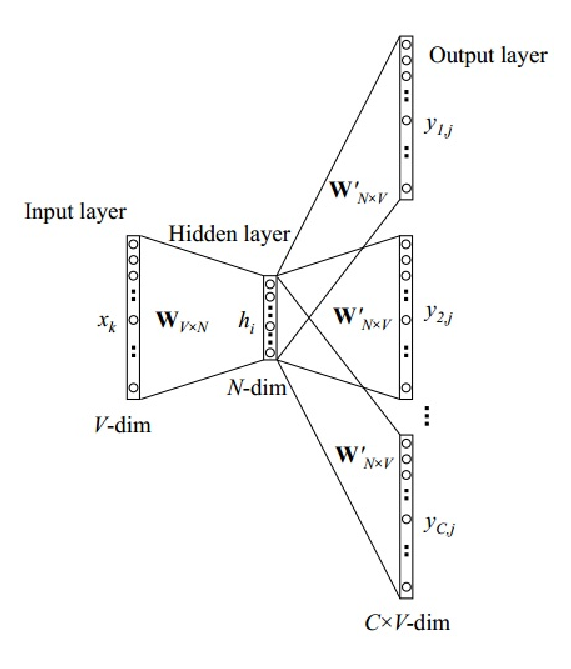
\includegraphics[width=70mm, height=70mm]{skipgram.eps}
\caption{Skip Gram Model(Figure from Rong (2014)) \label{fig:skipgram}}
\end{figure}

\subsection{tf-idf}
Let $D=d_1, d_2, d_3....d_N$ be $N$ documents under study and $T=t_1, t_2, t_3,....t_M$ be the $M$ unique terms in these documents, then each document can be represented as a $M$-dimensional vector:\\
$t_d=\{tf_1,tf_2,tf_3,...tf_M\}$\\
$tf-idf$ weights discounts the frequency of terms based on their importance to a particular document in the entire document set collection under consideration. This is done as follows:
\begin{center}
$tfidf(d,t)=tf(d,t) \times \log(\frac{|D|}{df(t)})$ 
\end{center}
Here $df(t)$ is the number of documents in which term $t$ appears.

\subsection{Vector Averaging for phrases}
	\label{sec:vectoraveraging}
As an output of the word vector learning, we now have a $n$-dimensional
vector representation for each word in the Hindi corpus.  Now we need to
assign features for sentences and paragraphs taken from the sentiment dataset
(training and test).  Mikolov et al. (2013b) and Levy et al. (2014) show that
many relational similarities can be recovered by means of vector arithmetic
in the embedded space.  Thus, additive models are useful, though
others have claimed that multiplicative models correlate better with human
judgments~\cite{Mitchell:08,Socher:13}.  In this work, we have retained teh
simplicity of vector averaging to model larger chunks of  discourse.
This models the sentence/document in the same high dimensional space.

A preprocessing step involved removing some words that appear at very high or
very low frequencies in the corpus.  
Our model was trained on the Hindi Wikipedia dump to create vector
representations for words. The previous two vectors were concatenated to
create another feature set for training purpose.  
%?? SIZE of wikipedia corpus, number of independent words etc. 

\underline{\emph{Algorithm}}
\begin{enumerate}
%\setlength{\itemsep}{0.5pt}
\item Input the Hindi text corpus
\item Train skip-gram model to obtain word vector representation
\item Given a sentiment training set, obtain average vector data for each sentence/document
\item Obtain tf-idf vector for each sentence/document in the corpus
\item Concatenate vectors of step 3 and step 4 to obtain a feature set for a training instance
\item Train linear SVM with $m$-fold cross validation to create a classifier
(here $m$=20)
\end{enumerate}
